\documentclass[tikz,border=2pt]{standalone}
\usepackage{amsmath,amssymb}
\usepackage{pgfplots}
\pgfplotsset{compat=1.18}
\usetikzlibrary{arrows.meta}

\begin{document}
% f(x) = x^3 - x on [a, b] = [-2, 2]: secant slope (f(2) - f(-2))/4 = 3 (secant y = 3x).
% f'(c) = 3c^2 - 1 = 3 at c = +-2/sqrt(3) = +-1.1547, f(c) = +-0.3849; tangents y = 3x -+ 3.0792.
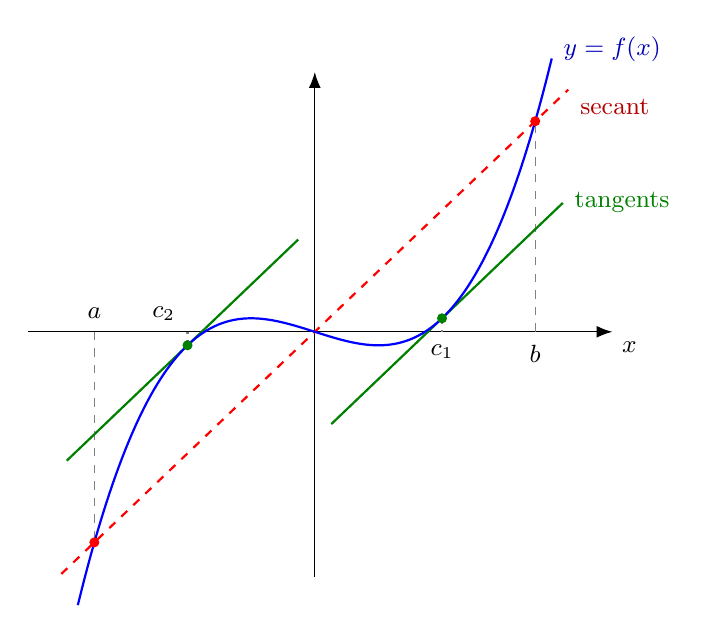
\begin{tikzpicture}[every node/.style={font=\small}]
	\begin{axis}[
		width=9cm, height=8cm,
		axis lines=middle, axis line style={-{Latex[length=2mm]}},
		xmin=-2.6, xmax=2.7, ymin=-7, ymax=7.4,
		xtick=\empty, ytick=\empty,
		xlabel={$x$}, xlabel style={below right},
		samples=150, clip=false
		]
		\addplot[gray, dashed] coordinates {(-2,0) (-2,-6)};
		\addplot[gray, dashed] coordinates {(2,0) (2,6)};
		\addplot[gray, dotted, thick] coordinates {(1.1547,0) (1.1547,0.3849)};
		\addplot[gray, dotted, thick] coordinates {(-1.1547,0) (-1.1547,-0.3849)};
		\addplot[red, dashed, thick, domain=-2.3:2.3] {3*x};
		\addplot[green!50!black, thick, domain=0.15:2.25] {3*x-3.0792};
		\addplot[green!50!black, thick, domain=-2.25:-0.15] {3*x+3.0792};
		\addplot[blue, thick, domain=-2.15:2.15] {x^3-x};
		\addplot[only marks, mark=*, mark size=1.6pt, red] coordinates {(-2,-6) (2,6)};
		\addplot[only marks, mark=*, mark size=1.6pt, green!50!black] coordinates {(1.1547,0.3849) (-1.1547,-0.3849)};
		\node[anchor=south, font=\small] at (axis cs:-2,0.1) {$a$};
		\node[anchor=north, font=\small] at (axis cs:2,-0.1) {$b$};
		\node[anchor=north, font=\small] at (axis cs:1.1547,-0.1) {$c_1$};
		\node[anchor=south east, font=\small] at (axis cs:-1.18,0.05) {$c_2$};
		\node[blue!70!black, anchor=west] at (axis cs:2.17,{2.17^3-2.17}) {$y=f(x)$};
		\node[red!70!black, anchor=west] at (axis cs:2.32,6.4) {secant};
		\node[green!50!black, anchor=west] at (axis cs:2.27,3.7) {tangents};
	\end{axis}
\end{tikzpicture}
\end{document}
